\section{Симметричные протоколы}
\selectlanguage{russian}

К симметричным будем относить протоколы, которые используют примитивы только классической криптографии на секретных ключах. К таким относятся уже известные блочные шифры, криптографически стойкие генераторы псевдослучайных чисел (КСГПСЧ) и хэш-функции.

При рассмотрении протоколов будем использовать следующие обозначения.
\begin{itemize}
	\item \textit{Alice}, \textit{Bob} -- легальные абоненты сети, для которых формируется общий сеансовый ключ. Алиса является инициатором.
	\item \textit{Trent} -- доверенный центр сети.
	\item $A$, $B$ -- некоторые идентификаторы легальных абонентов Алисы и Боба соответственно.
	\item $E_A$, $E_B$ -- результат шифрования некоторого блока данных с использованием секретных ключей легальных абонентов сети Алисы и Боба соответственно. Такое шифрование могу осуществить либо сами легальные абоненты, либо доверенный центр, которому известны все секретные ключи.
	\item $R_A$, $R_B$, $R_T$ -- случайные числа, генерируемые Алисой, Бобом и Трентом соответственно.
	\item $T_A$, $T_B$, $T_T$ -- метки времени, генерируемые Алисой, Бобом и Трентом соответственно.
	\item $K$ -- секретный сеансовый ключ, получение которого и является одной из целью протоколов.
\end{itemize}

\subsection{Протокол Wide-Mouth Frog}\index{протокол!Wide-Mouth Frog|(}
Протокол Wide-Mouth Frog является, возможно, самым простым протоколом с доверенным центром. Его автором считается Майкл Бэрроуз (1989 год, \langen{Michael Burrows},  \cite{Burrows:Abadi:Needham:1990}). Протокол состоит из следующих шагов.

\begin{figure}[!htb]
    \centering
    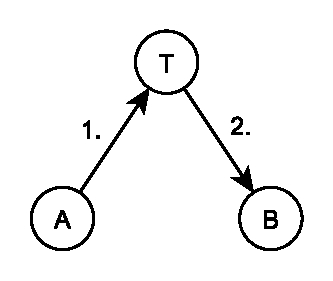
\includegraphics[width=0.5\textwidth]{pic/key_distribution-wide-mouth_frog}
    \caption{Схема взаимодействия абонентов и доверенного центра в протоколе Wide-Mouth Frog\label{fig:key_distribution-wide-mouth_frog}}
\end{figure}

\begin{enumerate}
	\item Алиса генерирует новый сеансовый ключ $K$ и отправляет его вместе с меткой времени, идентификатором Боба и своим незашифрованным идентификатором доверенному центру:
	\[ Alice \rightarrow \{ A, E_A \left( T_A, B, K \right) \} \rightarrow Trent \]
	\item Доверенный центр, используя полученный незашифрованный идентификатор $A$, находит у себя в базе данных легальных абонентов секретный ключ Алисы и расшифровывает им пакет данных. Проверяет метку времени (что пакет не очень старый). Далее он отправляет похожий пакет данных Бобу, зашифрованный его секретным ключом:
	\[ Trent \rightarrow \{ E_B \left( T_T, A, K \right) \} \rightarrow Bob \]
	Боб, кроме расшифрования пакета, также проверяет метку времени доверенного центра.
\end{enumerate}

По окончании протокола у Алисы и Боба есть общий сеансовый ключ $K$.

У данного протокола множество недостатков.

\begin{itemize}
	\item Генератором ключа является инициирующий абонент. Если предположить, что Боб -- это сервер, предоставляющий некоторый сервис, а Алиса -- это тонкий клиент, запрашивающий данный сервис, получается, что задача генерации надёжного сессионного ключа взваливается на плечи абонента с наименьшими мощностями.
	\item В протоколе общение с вызываемым абонентом происходит через доверенный центр. Как следствие, второй абонент может стать мишенью для DDOS-атаки с отражением (\langen{distributed denial-of-service attack}), когда злоумышленник будет посылать пакеты на доверенный центр, а тот формировать новые пакеты и посылать их абоненту. Если абонент подключён к нескольким сетям (с несколькими доверенными центрами), это позволит злоумышленнику вывести абонента из строя. Хотя защититься от подобной атаки достаточно просто, настроив соответствующим образом доверенный центр.
\end{itemize}

Однако самой серьёзной проблемой протокола является возможность применения следующих атак.

В 1995 году Рос Андерсон и Роджер Нидхем (\langen{Ross Anderson, Roger Needham}, \cite{Anderson:Needham:1995}) предложили вариант атаки на протокол, при котором злоумышленник (Ева) может бесконечно продлевать срок действия конкретного сеансового ключа. Идея атаки в том, что после окончания протокола злоумышленник будет посылать доверенному центру назад его же пакеты, дополняя их идентификаторами якобы инициирующего абонента.

\begin{enumerate}
	\item $ Alice \rightarrow \{ A, E_A \left( T_A, B, K \right) \} \rightarrow Trent $
	\item $ Trent \rightarrow \{ E_B \left( T_T, A, K \right) \} \rightarrow Bob $
	\item $ Eva \rightarrow \{ B, E_B \left( T_A, A, K \right) \} \rightarrow Trent $
	\item $ Trent \rightarrow \{ E_A \left( T'_T, B, K \right) \} \rightarrow Alice $
	\item $ Eva \rightarrow \{ A, E_A \left( T'_T, B, K \right) \} \rightarrow Trent $
	\item $ Trent \rightarrow \{ E_B \left( T''_T, A, K \right) \} \rightarrow Bob $
	\item Повторять шаги 3 и 5, пока не пройдёт время, нужное для получения $K$.
\end{enumerate}}

С точки зрения доверенного центра, шаги 1, 3 и 5 являются корректными пакетами, инициирующими общение абонентов между собой. Метки времени в них корректны (если Ева будет успевать вовремя эти пакеты посылать). С точки зрения легальных абонентов каждый из пакетов является приглашением другого абонента начать общение. В результате произойдёт две вещи:

\begin{itemize}
	\item Каждый из абонентов будет уверен, что закончился протокол создания нового сеансового ключа, что второй абонент успешно аутентифицировал себя перед доверенным центром. И что для установления следующего сеанса связи будет использоваться новый (на самом деле -- старый) ключ $K$.
	\item После того, как пройдёт время, нужное злоумышленнику Еве для взлома сеансового ключа $K$, Ева сможет и читать всю переписку, проходящую между абонентами, и успешно выдавать себя за обоих из абонентов.
\end{itemize}

Вторая атака 1997 года Гэвина Лоу (\langen{Gavin Lowe}, \cite{Lowe:1997}) проще в реализации. В результате этой атаки Боб уверен, что Алиса аутентифицировала себя перед доверенным центром и хочет начать второй сеанс общения. Что, конечно, не является правдой, так как второй сеанс инициирован злоумышленником.

\begin{enumerate}
	\item $ Alice \rightarrow \{ A, E_A \left( T_A, B, K \right) \} \rightarrow Trent $
	\item $ Trent \rightarrow \{ E_B \left( T_T, A, K \right) \} \rightarrow Bob $
	\item $ Eva \rightarrow \{ E_B \left( T_T, A, K \right) \} \rightarrow Bob $
\end{enumerate}

В той же работе Лоу предложил модификацию протокола, вводящую явную взаимную аутентификацию абонентов с помощью случайной метки $R_B$ и проверки, что Алиса может расшифровать пакет с меткой, зашифрованной общим сеансовым ключом абонентов $K$. Однако данная модификация приводит к тому, что протокол теряет своё самое главное преимущество перед другими протоколами -- простоту.

\begin{enumerate}
	\item $ Alice \rightarrow \{ A, E_A \left( T_A, B, K \right) \} \rightarrow Trent $
	\item $ Trent \rightarrow \{ E_B \left( T_T, A, K \right) \} \rightarrow Bob $
	\item $ Bob \rightarrow \{ E_K \left( R_B \right) \} \rightarrow Alice $
	\item $ Alice \rightarrow \{ E_K \left( R_B + 1 \right) \} \rightarrow Bob $
\end{enumerate}

\index{протокол!Wide-Mouth Frog|)}


\subsection{Протокол Нидхема~---~Шрёдера}\index{протокол!Нидхема~---~Шрёдера|(}
\selectlanguage{russian}

Протокол Нидхема~---~Шрёдера (\langen{Roger Needham, Michael Shroeder}, 1979,~\cite{Needham:Schroeder:1978}) похож на модифицированный протокол Wide-Mouth Frog, но отличается тем, что доверенный центр (Трент) во время работы основной части протокола не общается со вторым абонентом. Первый абонент получает от доверенного центра специальный пакет, который он без всякой модификации отправляет второму абоненту.

\begin{figure}[!htb]
    \centering
    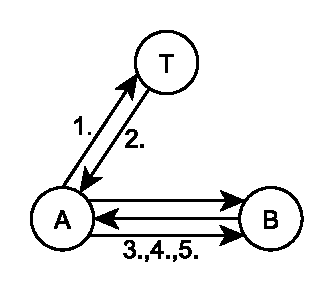
\includegraphics[width=0.5\textwidth]{pic/key_distribution-needham-schroeder}
    \caption{Схема взаимодействия абонентов и доверенного центра в протоколе Нидхема~---~Шрёдера\label{fig:key_distribution-needham-schroeder}}
\end{figure}

\begin{enumerate}
	\item $ Alice	\rightarrow \{ A, B, R_A \}						\rightarrow Trent $
	\item $ Trent	\rightarrow \{ E_A \left( R_A, B, K, E_B \left( K, A \right) \right) \}	\rightarrow Alice $
	\item $ Alice	\rightarrow \{ E_B \left( K, A \right) \}				\rightarrow Bob $
	\item $ Bob	\rightarrow \{ E_K \left( R_B \right) \}				\rightarrow Alice $
	\item $ Alice	\rightarrow \{ E_K \left( R_B - 1 \right) \}				\rightarrow Bob $
\end{enumerate}

Протокол обеспечивает и двустороннюю аутентификацию сторон, и, казалось бы, защиту от атак с повторной передачей (\langen{replay attack}). Последнее делается с помощью введения уже известных по модифицированному протоколу Wide-Mouth Frog случайных меток $R_A$ и $R_B$. Действительно, без знания ключа злоумышленник не сможет выдать себя за Алису перед Бобом (так как не сможет расшифровать пакет с зашифрованной меткой $R_B$). Однако, как мы договорились ранее во введении к этой главе, сам сессионный ключ не может считаться надёжным длительное время. Если злоумышленник сумеет в какой-то момент времени получить ранее использованный сессионный ключ $K$, он сможет убедить Боба, что он является Алисой, и что это новый сессионный ключ. Для этого ему понадобится переданный ранее по открытому каналу пакет из пункта 3 протокола.

\begin{enumerate}
	\item $ Eva		\rightarrow \{ A, B, R_A \}						\rightarrow Trent $
	\item $ Trent		\rightarrow \{ E_A \left( R_A, B, K, E_B \left( K, A \right) \right) \}	\rightarrow Alice $
	\item $ Alice		\rightarrow \{ E_B \left( K, A \right) \}				\rightarrow Bob $
	\item $ Bob		\rightarrow \{ E_K \left( R_B \right) \}				\rightarrow Alice $
	\item $ Alice		\rightarrow \{ E_K \left( R_B - 1 \right) \}				\rightarrow Bob $

		$\dots$ по прошествии некоторого времени $\dots$\\
	\item $ Eva~(Alice)	\rightarrow \{ E_B \left( K, A \right) \}				\rightarrow Bob $
	\item $ Bob		\rightarrow \{ E_K \left( R_B \right) \}				\rightarrow Eva~(Alice) $
	\item $ Eva (Alice)	\rightarrow \{ E_K \left( R_B - 1 \right) \}				\rightarrow Bob $
\end{enumerate}

Относительно мелкий недостаток протокола состоит ещё и в том, что во втором пакете доверенный центр в зашифрованном виде передаёт то, что в третьем шаге пересылается по открытому каналу ($E_B \left( K, A \right)$).

Если в протокол добавить метки времени, тем самым ограничив время возможного использования сессионного ключа, а также исправить мелкий недостаток с двойным шифрованием, можно получить протокол, который лежит в основе распространённого средства аутентификации <<Kerberos>> для локальных сетей.

\index{протокол!Нидхема~---~Шрёдера|)}


\subsection{Протокол <<Kerberos>>}\index{протокол!Kerberos|(}
\selectlanguage{russian}

В данном разделе будет описан протокол аутентификации сторон с единственным доверенным центром. Сетевой протокол <<Kerberos>> использует эти идеи при объединении нескольких доверенных центров в единую сеть для обеспечения надёжности и отказоустойчивости. Подробнее о сетевом протоколе <<Kerberos>> смотрите в разделе~\ref{section-kerberos}.

Как и в протоколе Нидхема~---~Шрёдера, инициирующий абонент (Алиса) общается только с выделенным доверенным центром, получая от него два пакета с зашифрованным сессионным ключом -- один для себя, а второй -- для вызываемого абонента (Боба). Однако в отличие от Нидхема~---~Шрёдера в рассматриваемом протоколе зашифрованные пакеты содержат также метку времени $T_T$ и срок действия сессионного ключа $L$ (от \langen{lifetime} -- срок жизни). Что позволяет, во-первых, защититься от рассмотренной в предыдущем разделе атаки повтором. А, во-вторых, позволяет доверенному центру в некотором смысле управлять абонентами, заставляя их получать новые сессионные ключи по истечению заранее заданного времени $L$.

\begin{figure}[!htb]
    \centering
    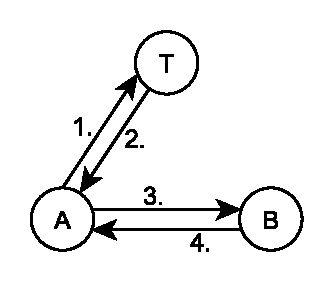
\includegraphics[width=0.5\textwidth]{pic/key_distribution-kerberos}
    \caption{Схема взаимодействия абонентов и доверенного центра в протоколе <<Kerberos>>\label{fig:key_distribution-kerberos}}
\end{figure}

\begin{enumerate}
	\item $ Alice	\rightarrow \{ A, B \}									\rightarrow Trent $
	\item $ Trent	\rightarrow \{ E_A \left( T_T, L, K, B \right), E_B \left( T_T, L, K, A \right) \}	\rightarrow Alice $
	\item $ Alice	\rightarrow \{ E_B \left( T_T, L, K, A \right), E_K \left( A, T_A \right) \}		\rightarrow Bob $
	\item $ Bob	\rightarrow \{ E_K \left( T_T + 1 \right) \}						\rightarrow Alice $
\end{enumerate}

Обратите внимание, что третий шаг за счёт использования метки времени от доверенного центра $T_T$ вместо случайной метки от Боба $R_B$ позволяет сократить протокол на один шаг по сравнению с протоколом Нидхема~---~Шрёдера. Также наличие метки времени делает ненужным и предварительную генерацию случайной метки Алисой и её передачу на первом шаге.

Интересно отметить, что пакеты $E_A \left( T_T, L, K, B \right)$ и $E_B \left( T_T, L, K, A \right)$ одинаковы по своему формату. В некотором смысле их можно назвать сертификатами сессионного ключа для Алисы и Боба. Причём все подобные пары пакетов можно сгенерировать заранее (например, в начале дня), выложить на общедоступный ресурс, предоставить в свободное использование и выключить доверенный центр (он своё дело уже сделал -- сгенерировав эти пакеты). И до момента времени $T_T + L$ этими <<сертификатами>> можно пользоваться. Но только если вы являетесь одной из допустимых пар абонентов. Конечно, эта идея непрактична -- ведь количество таких пар растёт как квадрат от числа абонентов. Однако интересен тот факт, что подобные пакеты можно сгенерировать заранее. Эта идея нам пригодится при рассмотрении инфраструктуры открытых ключей (\langen{public key infrastructure, PKI}).

\index{протокол!Kerberos|)}
